\documentclass[11pt,a4paper]{article}
\usepackage[margin=1.9cm, top=2.1cm, bottom=2.0cm]{geometry}
\usepackage[T1]{fontenc}
\usepackage{lmodern}
\usepackage{amsmath,amssymb}
\usepackage{enumitem,booktabs,array,tabularx,multirow}
\usepackage[normalem]{ulem}
\usepackage{adjustbox}
\usepackage{xcolor}
\usepackage{fancyhdr,lastpage}
\usepackage[most]{tcolorbox}
\usepackage{tikz}
\usetikzlibrary{shapes.geometric,arrows.meta,positioning,calc}
\usepackage[hidelinks]{hyperref}
\setlength{\parindent}{0pt}
\setlength{\parskip}{4pt}
\renewcommand{\arraystretch}{1.25}
\emergencystretch=2em
\pagestyle{fancy}\fancyhf{}
\lhead{\small\textit{Course: CS420 -- Artificial Intelligence}}
\rhead{\small Practice Test 4}
\cfoot{\small Page \thepage\ of \pageref{LastPage}}
\renewcommand{\headrulewidth}{0.4pt}
% empty answer box (exam) / filled box (solution)
\newtcolorbox{ansbox}[1][]{enhanced, breakable, colback=white, colframe=black!55, boxrule=0.5pt, arc=0pt,
  left=5pt, right=5pt, top=3pt, bottom=3pt, before skip=3pt, after skip=6pt, #1}
\newtcolorbox{solbox}{enhanced, breakable, colback=blue!2!white, colframe=blue!50!black, boxrule=0.6pt, arc=0pt,
  left=6pt, right=6pt, top=4pt, bottom=4pt, before skip=3pt, after skip=8pt,
  fontupper=\color{black}}
\newcommand{\question}[1]{\par\medskip\noindent\textbf{Question #1.}\ }
\newcommand{\subq}[1]{\par\smallskip\noindent\textbf{#1}\ }
\newcommand{\T}{\textbf{\textcolor{green!45!black}{TRUE}}}
\newcommand{\F}{\textbf{\textcolor{red!70!black}{FALSE}}}

\tikzset{
  maxn/.style={draw, thick, regular polygon, regular polygon sides=3, minimum size=10.5mm, inner sep=0pt, font=\small},
  minn/.style={maxn, shape border rotate=180},
  chn/.style={draw, thick, circle, minimum size=9.5mm, inner sep=0pt, font=\small},
  leafn/.style={draw, rectangle, minimum width=5.5mm, minimum height=5.5mm, inner sep=1pt, font=\small},
  gone/.style={draw=black!25, text=black!35},
  cut/.style={red!80!black, very thick, dashed},
  sol/.style={text=blue!70!black, font=\small\bfseries},
}

\begin{document}


{\large\textbf{\textit{Course: CS420 -- Artificial Intelligence}}}\par
{\textbf{\textit{Midterm examination review -- Lectures 0 to 3}}}\par
\begin{center}{\Large\bfseries PRACTICE MIDTERM EXAMINATION -- TEST 4}\\[3pt]
{\small Duration: 120 minutes \quad$\cdot$\quad Closed book \quad$\cdot$\quad Calculator allowed}\end{center}
\noindent\rule{\linewidth}{0.6pt}

\noindent Full name: \rule{6.5cm}{0.3pt}\hfill Student ID: \rule{4cm}{0.3pt}\par\smallskip
{\small\textit{Unless a question says otherwise, ties are broken in alphabetical order (left-to-right in trees), and successors are generated in alphabetical order.}}\par
\question{1}\textit{Vacuum world with three cells.} A vacuum-cleaner robot lives in a row of \textbf{three} cells (1, 2, 3). Each cell is either dirty or clean. The robot can move Left, move Right, or Suck (clean its current cell).
\subq{(a)}Consider a state as a tuple of values. Which values should be included in the tuple?
\begin{ansbox}[height=0.9cm]\end{ansbox}
\subq{(b)}Define the initial state (robot in cell 1, all cells dirty) and the goal state(s).
\begin{ansbox}[height=0.9cm]\end{ansbox}
\subq{(c)}Define the action function. What happens when moving Left in cell 1, Right in cell 3, or Sucking a clean cell?
\begin{ansbox}[height=1.4cm]\end{ansbox}
\subq{(d)}What is the action cost?
\begin{ansbox}[height=0.6cm]\end{ansbox}
\subq{(e)}What is the maximum number of states? How many are reachable from the initial state? Give a shortest solution.
\begin{ansbox}[height=1.4cm]\end{ansbox}
\question{2}Consider the undirected graph below with initial state $S$ and \textbf{two} goal states $G_1$, $G_2$; a search stops at whichever goal satisfies its goal test first. \begin{center}
\begin{adjustbox}{max width=\linewidth}
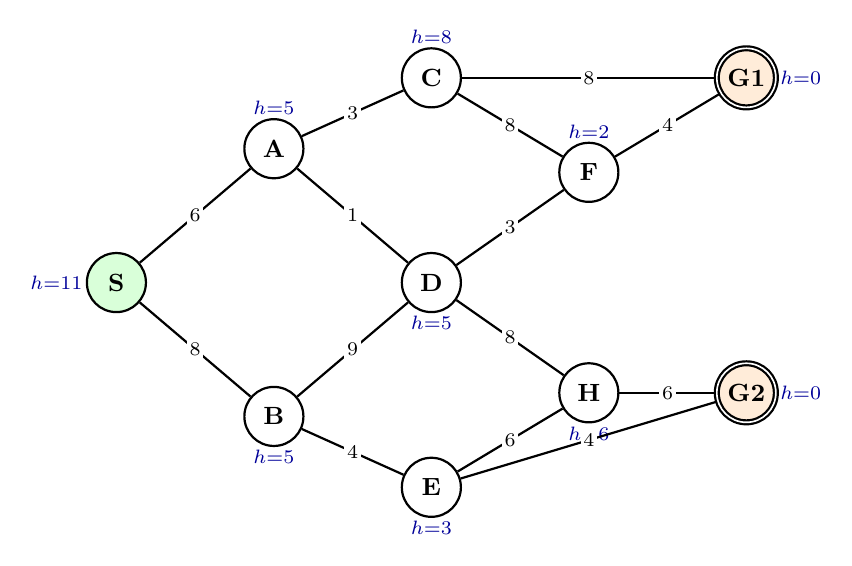
\begin{tikzpicture}[scale=1.0, every node/.style={transform shape}, gn/.style={draw, thick, circle, minimum size=7.5mm, inner sep=0pt, font=\small\bfseries}, ec/.style={font=\scriptsize, fill=white, inner sep=1pt}]
\node[gn, fill=green!15, label={[font=\scriptsize, text=blue!60!black, inner sep=1pt]left:$h{=}11$}] (S) at (0.00,0.00) {S};
\node[gn, label={[font=\scriptsize, text=blue!60!black, inner sep=1pt]above:$h{=}5$}] (A) at (2.00,1.70) {A};
\node[gn, label={[font=\scriptsize, text=blue!60!black, inner sep=1pt]below:$h{=}5$}] (B) at (2.00,-1.70) {B};
\node[gn, label={[font=\scriptsize, text=blue!60!black, inner sep=1pt]above:$h{=}8$}] (C) at (4.00,2.60) {C};
\node[gn, label={[font=\scriptsize, text=blue!60!black, inner sep=1pt]below:$h{=}5$}] (D) at (4.00,0.00) {D};
\node[gn, label={[font=\scriptsize, text=blue!60!black, inner sep=1pt]below:$h{=}3$}] (E) at (4.00,-2.60) {E};
\node[gn, label={[font=\scriptsize, text=blue!60!black, inner sep=1pt]above:$h{=}2$}] (F) at (6.00,1.40) {F};
\node[gn, label={[font=\scriptsize, text=blue!60!black, inner sep=1pt]below:$h{=}6$}] (H) at (6.00,-1.40) {H};
\node[gn, double, fill=orange!15, label={[font=\scriptsize, text=blue!60!black, inner sep=1pt]right:$h{=}0$}] (G1) at (8.00,2.60) {G1};
\node[gn, double, fill=orange!15, label={[font=\scriptsize, text=blue!60!black, inner sep=1pt]right:$h{=}0$}] (G2) at (8.00,-1.40) {G2};
\draw[thick] (S) to[] node[ec, midway]{6} (A);
\draw[thick] (S) to[] node[ec, midway]{8} (B);
\draw[thick] (A) to[] node[ec, midway]{3} (C);
\draw[thick] (A) to[] node[ec, midway]{1} (D);
\draw[thick] (B) to[] node[ec, midway]{9} (D);
\draw[thick] (B) to[] node[ec, midway]{4} (E);
\draw[thick] (C) to[] node[ec, midway]{8} (F);
\draw[thick] (C) to[] node[ec, midway]{8} (G1);
\draw[thick] (D) to[] node[ec, midway]{3} (F);
\draw[thick] (D) to[] node[ec, midway]{8} (H);
\draw[thick] (E) to[] node[ec, midway]{6} (H);
\draw[thick] (F) to[] node[ec, midway]{4} (G1);
\draw[thick] (H) to[] node[ec, midway]{6} (G2);
\draw[thick] (E) to[] node[ec, midway]{4} (G2);
\end{tikzpicture}
\end{adjustbox}
\end{center}For each search strategy, (a) list, in order, the states \textbf{expanded}, (b) give the path found and (c) give the final content of the frontier (a state is expanded when it is removed from the frontier). Conventions: BFS, DFS and greedy best-first search test a state for the goal when it is \emph{generated} (so the goal is not expanded); UCS and A* test it when it is \emph{removed} from the frontier (graph search; a cheaper path to a frontier state replaces its entry). DFS avoids loops by remembering the states on the current path only. The path returned will not be accepted if the list of expanded states is wrong.

\begin{center}\small\begin{tabularx}{\linewidth}{|>{\raggedright}p{2.6cm}|>{\raggedright}X|>{\raggedright}p{3.6cm}|>{\raggedright\arraybackslash}p{2.6cm}|}\hline
\textbf{Algorithm} & \textbf{List of expanded states} & \textbf{Path returned} & \textbf{Final frontier}\\ \hline
Breadth-first search & & & \\[8mm] \hline
Uniform-cost search & & & \\[8mm] \hline
Depth-first search & & & \textit{(not asked)}\\[8mm] \hline
Greedy best-first search & & & \\[8mm] \hline
Graph-search A* & & & \\[8mm] \hline
\end{tabularx}\end{center}
\subq{(d)}With several goals, what must an admissible heuristic estimate? Is $h$ admissible and consistent?
\begin{ansbox}[height=1.6cm]\end{ansbox}
\subq{(e)}Which goal does each strategy reach? Why does greedy best-first search end at a different goal from A*?
\begin{ansbox}[height=1.8cm]\end{ansbox}
\clearpage
\question{3}Consider the 8-puzzle. Apply \emph{steepest-descent hill climbing} with the Manhattan-distance heuristic $h$ to the following pair of initial and goal states.\begin{center}Initial state\quad \begin{tabular}{|c|c|c|}\hline 1 & 2 & 5\\\hline 3 & -- & 4\\\hline 6 & 7 & 8\\\hline\end{tabular}\qquad\qquad Goal state\quad \begin{tabular}{|c|c|c|}\hline -- & 1 & 2\\\hline 3 & 4 & 5\\\hline 6 & 7 & 8\\\hline\end{tabular}\end{center}Your work should: draw the search tree including all successors of every expanded state (moves of the blank in the order Up, Down, Left, Right; do not regenerate the parent state), write the heuristic value of every node, and mark the path found.
\par\smallskip\noindent 
\begin{ansbox}[height=12.0cm]\end{ansbox}
\clearpage
\question{4}Consider the following game tree (MAX at the root).\begin{center}
\begin{adjustbox}{max width=\linewidth}
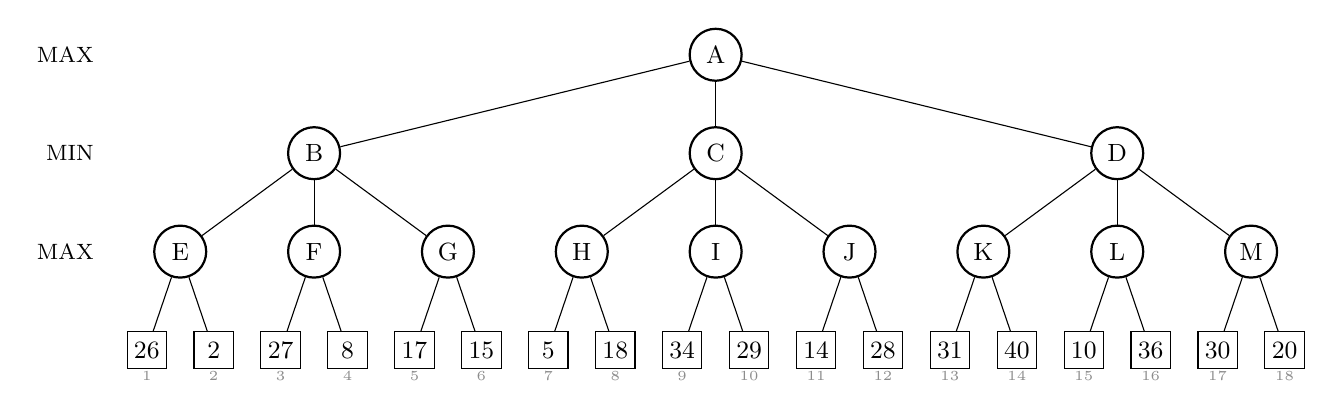
\begin{tikzpicture}[scale=1.0, every node/.style={transform shape}, gc/.style={draw, thick, circle, minimum size=6.6mm, inner sep=0pt, font=\small}, gl/.style={draw, rectangle, minimum width=5mm, minimum height=4.6mm, inner sep=1pt, font=\small}, gx/.style={draw=black!25, text=black!35}, val/.style={font=\footnotesize\bfseries, text=red!80!black, inner sep=1pt}]
\node[font=\footnotesize, anchor=east] at (-0.55,0.00) {MAX};
\node[font=\footnotesize, anchor=east] at (-0.55,-1.25) {MIN};
\node[font=\footnotesize, anchor=east] at (-0.55,-2.50) {MAX};
\node[gc] (n30) at (7.225,0.000) {A};
\node[gc] (n9) at (2.125,-1.250) {B};
\node[gc] (n2) at (0.425,-2.500) {E};
\node[gl, label={[font=\tiny, text=black!45, inner sep=1pt]below:1}] (n0) at (0.000,-3.750) {26};
\node[gl, label={[font=\tiny, text=black!45, inner sep=1pt]below:2}] (n1) at (0.850,-3.750) {2};
\node[gc] (n5) at (2.125,-2.500) {F};
\node[gl, label={[font=\tiny, text=black!45, inner sep=1pt]below:3}] (n3) at (1.700,-3.750) {27};
\node[gl, label={[font=\tiny, text=black!45, inner sep=1pt]below:4}] (n4) at (2.550,-3.750) {8};
\node[gc] (n8) at (3.825,-2.500) {G};
\node[gl, label={[font=\tiny, text=black!45, inner sep=1pt]below:5}] (n6) at (3.400,-3.750) {17};
\node[gl, label={[font=\tiny, text=black!45, inner sep=1pt]below:6}] (n7) at (4.250,-3.750) {15};
\node[gc] (n19) at (7.225,-1.250) {C};
\node[gc] (n12) at (5.525,-2.500) {H};
\node[gl, label={[font=\tiny, text=black!45, inner sep=1pt]below:7}] (n10) at (5.100,-3.750) {5};
\node[gl, label={[font=\tiny, text=black!45, inner sep=1pt]below:8}] (n11) at (5.950,-3.750) {18};
\node[gc] (n15) at (7.225,-2.500) {I};
\node[gl, label={[font=\tiny, text=black!45, inner sep=1pt]below:9}] (n13) at (6.800,-3.750) {34};
\node[gl, label={[font=\tiny, text=black!45, inner sep=1pt]below:10}] (n14) at (7.650,-3.750) {29};
\node[gc] (n18) at (8.925,-2.500) {J};
\node[gl, label={[font=\tiny, text=black!45, inner sep=1pt]below:11}] (n16) at (8.500,-3.750) {14};
\node[gl, label={[font=\tiny, text=black!45, inner sep=1pt]below:12}] (n17) at (9.350,-3.750) {28};
\node[gc] (n29) at (12.325,-1.250) {D};
\node[gc] (n22) at (10.625,-2.500) {K};
\node[gl, label={[font=\tiny, text=black!45, inner sep=1pt]below:13}] (n20) at (10.200,-3.750) {31};
\node[gl, label={[font=\tiny, text=black!45, inner sep=1pt]below:14}] (n21) at (11.050,-3.750) {40};
\node[gc] (n25) at (12.325,-2.500) {L};
\node[gl, label={[font=\tiny, text=black!45, inner sep=1pt]below:15}] (n23) at (11.900,-3.750) {10};
\node[gl, label={[font=\tiny, text=black!45, inner sep=1pt]below:16}] (n24) at (12.750,-3.750) {36};
\node[gc] (n28) at (14.025,-2.500) {M};
\node[gl, label={[font=\tiny, text=black!45, inner sep=1pt]below:17}] (n26) at (13.600,-3.750) {30};
\node[gl, label={[font=\tiny, text=black!45, inner sep=1pt]below:18}] (n27) at (14.450,-3.750) {20};
\draw (n30) -- (n9);
\draw (n30) -- (n19);
\draw (n30) -- (n29);
\draw (n9) -- (n2);
\draw (n9) -- (n5);
\draw (n9) -- (n8);
\draw (n2) -- (n0);
\draw (n2) -- (n1);
\draw (n5) -- (n3);
\draw (n5) -- (n4);
\draw (n8) -- (n6);
\draw (n8) -- (n7);
\draw (n19) -- (n12);
\draw (n19) -- (n15);
\draw (n19) -- (n18);
\draw (n12) -- (n10);
\draw (n12) -- (n11);
\draw (n15) -- (n13);
\draw (n15) -- (n14);
\draw (n18) -- (n16);
\draw (n18) -- (n17);
\draw (n29) -- (n22);
\draw (n29) -- (n25);
\draw (n29) -- (n28);
\draw (n22) -- (n20);
\draw (n22) -- (n21);
\draw (n25) -- (n23);
\draw (n25) -- (n24);
\draw (n28) -- (n26);
\draw (n28) -- (n27);
\end{tikzpicture}
\end{adjustbox}
\end{center}
\subq{(a)}Compute the final backed-up value of every node using the minimax algorithm (no alpha-beta pruning at this step). Which move should MAX make at the root?
\begin{center}\small \begin{tabular}{|l|c|c|c|c|c|c|c|c|c|c|c|c|c|}\hline
\textbf{Node} & \textbf{A} & \textbf{B} & \textbf{C} & \textbf{D} & \textbf{E} & \textbf{F} & \textbf{G} & \textbf{H} & \textbf{I} & \textbf{J} & \textbf{K} & \textbf{L} & \textbf{M}\\ \hline
Minimax & \phantom{00} & \phantom{00} & \phantom{00} & \phantom{00} & \phantom{00} & \phantom{00} & \phantom{00} & \phantom{00} & \phantom{00} & \phantom{00} & \phantom{00} & \phantom{00} & \phantom{00}\\[1.5mm] \hline
\end{tabular}\end{center}\begin{ansbox}[height=0.8cm]\end{ansbox}
\subq{(b)}Run alpha-beta pruning (children visited left to right). Give the value computed at every node (mark \textbf{X} if the node is never visited), cross out the pruned branches on the tree and briefly explain each case.
\begin{center}\small \begin{tabular}{|l|c|c|c|c|c|c|c|c|c|c|c|c|c|}\hline
\textbf{Node} & \textbf{A} & \textbf{B} & \textbf{C} & \textbf{D} & \textbf{E} & \textbf{F} & \textbf{G} & \textbf{H} & \textbf{I} & \textbf{J} & \textbf{K} & \textbf{L} & \textbf{M}\\ \hline
$\alpha$-$\beta$ & \phantom{00} & \phantom{00} & \phantom{00} & \phantom{00} & \phantom{00} & \phantom{00} & \phantom{00} & \phantom{00} & \phantom{00} & \phantom{00} & \phantom{00} & \phantom{00} & \phantom{00}\\[1.5mm] \hline
\end{tabular}\end{center}\begin{ansbox}[height=4.0cm]\end{ansbox}
\subq{(c)}Run alpha-beta again, this time visiting the children of every node from \textbf{right to left}. Which leaves are pruned now? Explain the difference.
\begin{ansbox}[height=4.0cm]\end{ansbox}
\clearpage
\question{5}Consider the game tree below, in which \textbf{MIN moves first}.\begin{center}
\begin{adjustbox}{max width=\linewidth}
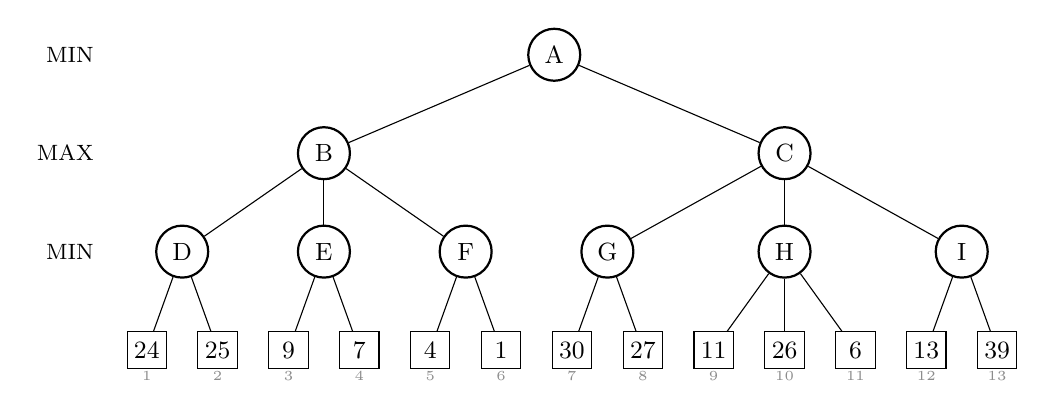
\begin{tikzpicture}[scale=1.0, every node/.style={transform shape}, gc/.style={draw, thick, circle, minimum size=6.6mm, inner sep=0pt, font=\small}, gl/.style={draw, rectangle, minimum width=5mm, minimum height=4.6mm, inner sep=1pt, font=\small}, gx/.style={draw=black!25, text=black!35}, val/.style={font=\footnotesize\bfseries, text=red!80!black, inner sep=1pt}]
\node[font=\footnotesize, anchor=east] at (-0.55,0.00) {MIN};
\node[font=\footnotesize, anchor=east] at (-0.55,-1.25) {MAX};
\node[font=\footnotesize, anchor=east] at (-0.55,-2.50) {MIN};
\node[gc] (n21) at (5.175,0.000) {A};
\node[gc] (n9) at (2.250,-1.250) {B};
\node[gc] (n2) at (0.450,-2.500) {D};
\node[gl, label={[font=\tiny, text=black!45, inner sep=1pt]below:1}] (n0) at (0.000,-3.750) {24};
\node[gl, label={[font=\tiny, text=black!45, inner sep=1pt]below:2}] (n1) at (0.900,-3.750) {25};
\node[gc] (n5) at (2.250,-2.500) {E};
\node[gl, label={[font=\tiny, text=black!45, inner sep=1pt]below:3}] (n3) at (1.800,-3.750) {9};
\node[gl, label={[font=\tiny, text=black!45, inner sep=1pt]below:4}] (n4) at (2.700,-3.750) {7};
\node[gc] (n8) at (4.050,-2.500) {F};
\node[gl, label={[font=\tiny, text=black!45, inner sep=1pt]below:5}] (n6) at (3.600,-3.750) {4};
\node[gl, label={[font=\tiny, text=black!45, inner sep=1pt]below:6}] (n7) at (4.500,-3.750) {1};
\node[gc] (n20) at (8.100,-1.250) {C};
\node[gc] (n12) at (5.850,-2.500) {G};
\node[gl, label={[font=\tiny, text=black!45, inner sep=1pt]below:7}] (n10) at (5.400,-3.750) {30};
\node[gl, label={[font=\tiny, text=black!45, inner sep=1pt]below:8}] (n11) at (6.300,-3.750) {27};
\node[gc] (n16) at (8.100,-2.500) {H};
\node[gl, label={[font=\tiny, text=black!45, inner sep=1pt]below:9}] (n13) at (7.200,-3.750) {11};
\node[gl, label={[font=\tiny, text=black!45, inner sep=1pt]below:10}] (n14) at (8.100,-3.750) {26};
\node[gl, label={[font=\tiny, text=black!45, inner sep=1pt]below:11}] (n15) at (9.000,-3.750) {6};
\node[gc] (n19) at (10.350,-2.500) {I};
\node[gl, label={[font=\tiny, text=black!45, inner sep=1pt]below:12}] (n17) at (9.900,-3.750) {13};
\node[gl, label={[font=\tiny, text=black!45, inner sep=1pt]below:13}] (n18) at (10.800,-3.750) {39};
\draw (n21) -- (n9);
\draw (n21) -- (n20);
\draw (n9) -- (n2);
\draw (n9) -- (n5);
\draw (n9) -- (n8);
\draw (n2) -- (n0);
\draw (n2) -- (n1);
\draw (n5) -- (n3);
\draw (n5) -- (n4);
\draw (n8) -- (n6);
\draw (n8) -- (n7);
\draw (n20) -- (n12);
\draw (n20) -- (n16);
\draw (n20) -- (n19);
\draw (n12) -- (n10);
\draw (n12) -- (n11);
\draw (n16) -- (n13);
\draw (n16) -- (n14);
\draw (n16) -- (n15);
\draw (n19) -- (n17);
\draw (n19) -- (n18);
\end{tikzpicture}
\end{adjustbox}
\end{center}
\subq{(a)}Note the minimax value of every node (no pruning).
\begin{center}\small \begin{tabular}{|l|c|c|c|c|c|c|c|c|c|}\hline
\textbf{Node} & \textbf{A} & \textbf{B} & \textbf{C} & \textbf{D} & \textbf{E} & \textbf{F} & \textbf{G} & \textbf{H} & \textbf{I}\\ \hline
Minimax & \phantom{00} & \phantom{00} & \phantom{00} & \phantom{00} & \phantom{00} & \phantom{00} & \phantom{00} & \phantom{00} & \phantom{00}\\[1.5mm] \hline
\end{tabular}\end{center}
\subq{(b)}Show where alpha-beta pruning occurs (left to right) by crossing out the corresponding branches, and briefly explain each case.
\begin{ansbox}[height=4.5cm]\end{ansbox}
\question{6}Three players A, B, C move in turn. Each leaf gives the utility vector $(u_A,u_B,u_C)$ and every player maximises its own component.\begin{center}
\begin{adjustbox}{max width=\linewidth}
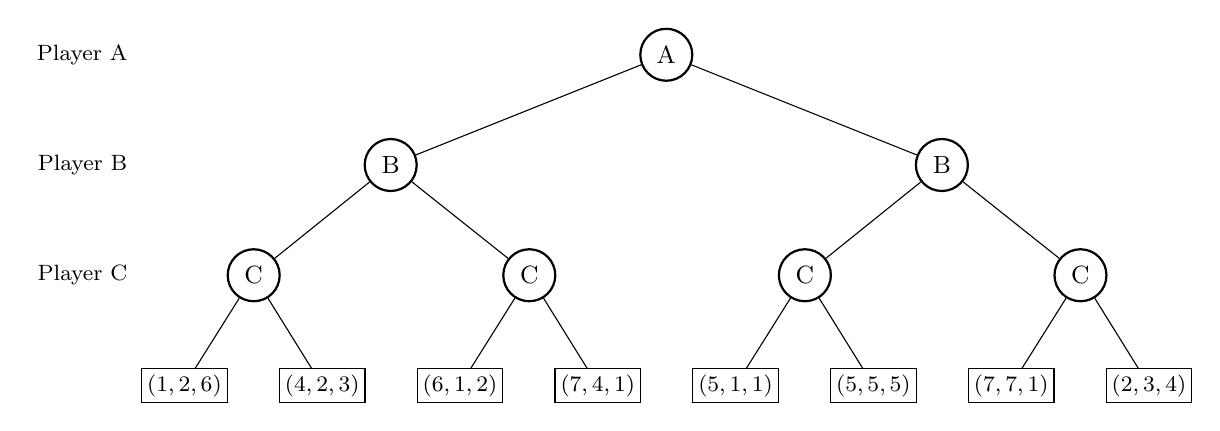
\begin{tikzpicture}[pn/.style={draw, thick, circle, minimum size=6.6mm, inner sep=0pt, font=\small}, lv/.style={draw, rectangle, inner sep=2pt, font=\footnotesize}]
\node[font=\footnotesize, anchor=east] at (-0.6,0.00) {Player A};
\node[font=\footnotesize, anchor=east] at (-0.6,-1.40) {Player B};
\node[font=\footnotesize, anchor=east] at (-0.6,-2.80) {Player C};
\node[pn] (p) at (6.12,0.00) {A};
\node[pn] (p0) at (2.62,-1.40) {B};
\node[pn] (p00) at (0.88,-2.80) {C};
\node[lv] (p000) at (0.00,-4.20) {$(1,2,6)$};
\draw (p00) -- (p000);
\node[lv] (p001) at (1.75,-4.20) {$(4,2,3)$};
\draw (p00) -- (p001);
\draw (p0) -- (p00);
\node[pn] (p01) at (4.38,-2.80) {C};
\node[lv] (p010) at (3.50,-4.20) {$(6,1,2)$};
\draw (p01) -- (p010);
\node[lv] (p011) at (5.25,-4.20) {$(7,4,1)$};
\draw (p01) -- (p011);
\draw (p0) -- (p01);
\draw (p) -- (p0);
\node[pn] (p1) at (9.62,-1.40) {B};
\node[pn] (p10) at (7.88,-2.80) {C};
\node[lv] (p100) at (7.00,-4.20) {$(5,1,1)$};
\draw (p10) -- (p100);
\node[lv] (p101) at (8.75,-4.20) {$(5,5,5)$};
\draw (p10) -- (p101);
\draw (p1) -- (p10);
\node[pn] (p11) at (11.38,-2.80) {C};
\node[lv] (p110) at (10.50,-4.20) {$(7,7,1)$};
\draw (p11) -- (p110);
\node[lv] (p111) at (12.25,-4.20) {$(2,3,4)$};
\draw (p11) -- (p111);
\draw (p1) -- (p11);
\draw (p) -- (p1);
\end{tikzpicture}
\end{adjustbox}
\end{center}
\subq{(a)}Back up the utility vectors to every node. Which move does A make?
\begin{ansbox}[height=1.4cm]\end{ansbox}
\subq{(b)}The game is not zero-sum. Explain, using this tree, why alliances may form and why they may be broken.
\begin{ansbox}[height=1.8cm]\end{ansbox}
\clearpage
\question{7}Consider the MCTS tree below; rewards are scores in $[0,10]$ for the root player. Use $\mathrm{UCB1}=\bar V_i+C\sqrt{\ln N/n_i}$ with $C=2$ (unvisited $=\infty$, ties to the left; a never-visited leaf is rolled out directly, otherwise all its children are added and the rollout starts at the first). Expansion: $A\to A_1,A_2,A_3$; $B\to B_1,B_2,B_3$; $X_i\to X_{i1},X_{i2}$; $X_{ij}\to X_{ij1},X_{ij2}$.\begin{center}
\begin{adjustbox}{max width=\linewidth}
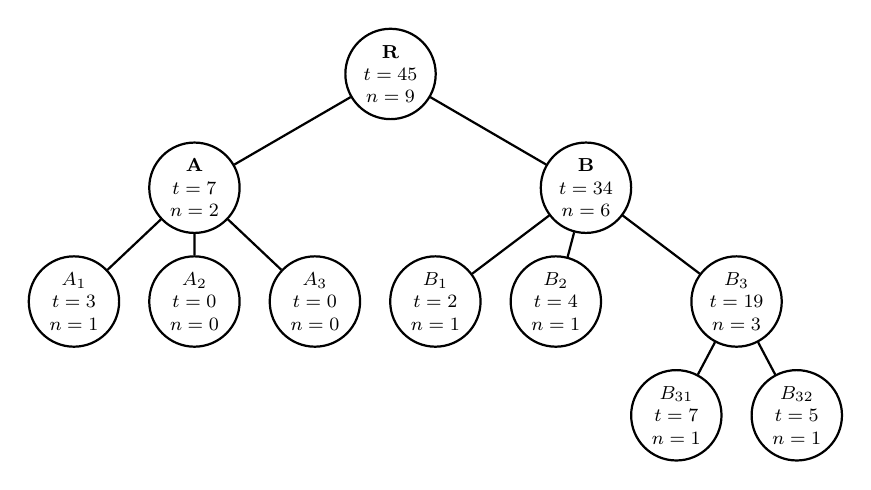
\begin{tikzpicture}[scale=0.85, every node/.style={transform shape}, mn/.style={draw, thick, circle, align=center, font=\footnotesize, inner sep=0.5pt, minimum size=13.5mm}]
\node[mn] (m1) at (4.73,0.00) {\textbf{R}\\ $t=45$\\ $n=9$};
\node[mn] (m2) at (1.80,-1.70) {\textbf{A}\\ $t=7$\\ $n=2$};
\node[mn] (m3) at (0.00,-3.40) {\textbf{$A_{1}$}\\ $t=3$\\ $n=1$};
\draw[thick] (m2) -- (m3);
\node[mn] (m4) at (1.80,-3.40) {\textbf{$A_{2}$}\\ $t=0$\\ $n=0$};
\draw[thick] (m2) -- (m4);
\node[mn] (m5) at (3.60,-3.40) {\textbf{$A_{3}$}\\ $t=0$\\ $n=0$};
\draw[thick] (m2) -- (m5);
\draw[thick] (m1) -- (m2);
\node[mn] (m6) at (7.65,-1.70) {\textbf{B}\\ $t=34$\\ $n=6$};
\node[mn] (m7) at (5.40,-3.40) {\textbf{$B_{1}$}\\ $t=2$\\ $n=1$};
\draw[thick] (m6) -- (m7);
\node[mn] (m8) at (7.20,-3.40) {\textbf{$B_{2}$}\\ $t=4$\\ $n=1$};
\draw[thick] (m6) -- (m8);
\node[mn] (m9) at (9.90,-3.40) {\textbf{$B_{3}$}\\ $t=19$\\ $n=3$};
\node[mn] (m10) at (9.00,-5.10) {\textbf{$B_{31}$}\\ $t=7$\\ $n=1$};
\draw[thick] (m9) -- (m10);
\node[mn] (m11) at (10.80,-5.10) {\textbf{$B_{32}$}\\ $t=5$\\ $n=1$};
\draw[thick] (m9) -- (m11);
\draw[thick] (m6) -- (m9);
\draw[thick] (m1) -- (m6);
\end{tikzpicture}
\end{adjustbox}
\end{center}
\subq{(a)}Perform three iterations whose rollouts return $0,\ 1,\ 10$ (in order). Give the UCB1 values at every selection step and draw the final tree.
\begin{ansbox}[height=9.0cm]\end{ansbox}
\subq{(b)}Which root action is chosen by the \emph{max child}, \emph{robust child} and \emph{secure child} rules (secure: maximise $\bar V_i-C\sqrt{\ln N/n_i}$, $C=2$)? What does \emph{max-robust child} recommend?
\begin{ansbox}[height=1.8cm]\end{ansbox}
\clearpage
\question{8}This problem is about map colouring. Each region must be coloured Red (R), Green (G) or Blue (B), and neighbouring regions must have different colours. The constraint graph is shown below. The following questions are mutually independent.\begin{center}
\begin{adjustbox}{max width=\linewidth}
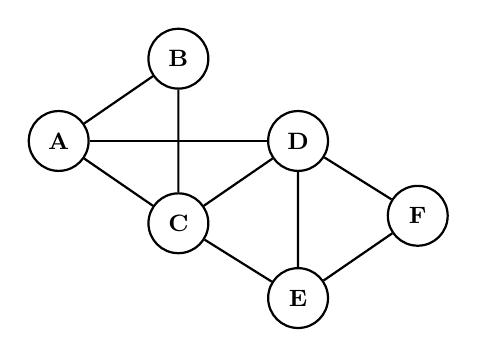
\begin{tikzpicture}[scale=0.95, every node/.style={transform shape}, cv/.style={draw, thick, circle, minimum size=8mm, inner sep=0pt, font=\small\bfseries}]
\node[cv] (A) at (0.00,1.10) {A};
\node[cv] (B) at (1.60,2.20) {B};
\node[cv] (C) at (1.60,0.00) {C};
\node[cv] (D) at (3.20,1.10) {D};
\node[cv] (E) at (3.20,-1.00) {E};
\node[cv] (F) at (4.80,0.10) {F};
\draw[thick] (A) to[] (B);
\draw[thick] (A) to[] (C);
\draw[thick] (A) to[] (D);
\draw[thick] (B) to[] (C);
\draw[thick] (C) to[] (D);
\draw[thick] (C) to[] (E);
\draw[thick] (D) to[] (E);
\draw[thick] (D) to[] (F);
\draw[thick] (E) to[] (F);
\end{tikzpicture}
\end{adjustbox}
\end{center}
\subq{(a)}\textbf{Cross out} all values that would be eliminated by \emph{forward checking} after variable B has been assigned as shown.\begin{center}\small\begin{tabular}{|l|c|c|c|c|c|c|}\hline Variables & \textbf{A} & \textbf{B} & \textbf{C} & \textbf{D} & \textbf{E} & \textbf{F}\\ \hline Domains & R\ G\ B & \textbf{R} & R\ G\ B & R\ G\ B & R\ G\ B & R\ G\ B\\ \hline\end{tabular}\end{center}

\subq{(b)}A and B have been assigned as shown, but no constraint propagation has been done yet. \textbf{Cross out} all values that would be eliminated by \emph{arc consistency} (AC-3).\begin{center}\small\begin{tabular}{|l|c|c|c|c|c|c|}\hline Variables & \textbf{A} & \textbf{B} & \textbf{C} & \textbf{D} & \textbf{E} & \textbf{F}\\ \hline Domains & \textbf{R} & \textbf{G} & R\ G\ B & R\ G\ B & R\ G\ B & R\ G\ B\\ \hline\end{tabular}\end{center}

\subq{(c)}Variable A is already assigned and constraint propagation has been done. \textbf{Circle} all unassigned variables that might be selected by the \emph{Minimum-Remaining-Values} (MRV) heuristic.\begin{center}\small\begin{tabular}{|l|c|c|c|c|c|c|}\hline Variables & \textbf{A} & \textbf{B} & \textbf{C} & \textbf{D} & \textbf{E} & \textbf{F}\\ \hline Domains & \textbf{R} & G\ B & G\ B & G\ B & R\ G\ B & R\ G\ B\\ \hline\end{tabular}\end{center}

\subq{(d)}Same situation. \textbf{Circle} all unassigned variables that might be selected by the \emph{Degree Heuristic}.\begin{center}\small\begin{tabular}{|l|c|c|c|c|c|c|}\hline Variables & \textbf{A} & \textbf{B} & \textbf{C} & \textbf{D} & \textbf{E} & \textbf{F}\\ \hline Domains & \textbf{R} & G\ B & G\ B & G\ B & R\ G\ B & R\ G\ B\\ \hline\end{tabular}\end{center}

\subq{(e)}Assume no variable has been assigned yet. Solve the CSP using backtracking with \emph{forward checking}, choosing variables with MRV, then the degree heuristic (DH), and finally alphabetical order; try values in the order R, G, B. For every step give the MRV value of every region not yet coloured, and the DH values of the regions tied on the minimum MRV.
\par \underline{Step 1}\par\begin{center}\small \begin{tabular}{|l|c|c|c|c|c|c|}\hline Variables & \textbf{A} & \textbf{B} & \textbf{C} & \textbf{D} & \textbf{E} & \textbf{F}\\ \hline MRV & \phantom{0} & \phantom{0} & \phantom{0} & \phantom{0} & \phantom{0} & \phantom{0}\\[1mm]\hline DH & \phantom{0} & \phantom{0} & \phantom{0} & \phantom{0} & \phantom{0} & \phantom{0}\\[1mm]\hline\end{tabular}\end{center}Assign to the variable \rule{2.5cm}{0.3pt} with the value \rule{2.5cm}{0.3pt}\par
\underline{Step 2}\par\begin{center}\small \begin{tabular}{|l|c|c|c|c|c|c|}\hline Variables & \textbf{A} & \textbf{B} & \textbf{C} & \textbf{D} & \textbf{E} & \textbf{F}\\ \hline MRV & \phantom{0} & \phantom{0} & \phantom{0} & \phantom{0} & \phantom{0} & \phantom{0}\\[1mm]\hline DH & \phantom{0} & \phantom{0} & \phantom{0} & \phantom{0} & \phantom{0} & \phantom{0}\\[1mm]\hline\end{tabular}\end{center}Assign to the variable \rule{2.5cm}{0.3pt} with the value \rule{2.5cm}{0.3pt}\par
\underline{Step 3}\par\begin{center}\small \begin{tabular}{|l|c|c|c|c|c|c|}\hline Variables & \textbf{A} & \textbf{B} & \textbf{C} & \textbf{D} & \textbf{E} & \textbf{F}\\ \hline MRV & \phantom{0} & \phantom{0} & \phantom{0} & \phantom{0} & \phantom{0} & \phantom{0}\\[1mm]\hline DH & \phantom{0} & \phantom{0} & \phantom{0} & \phantom{0} & \phantom{0} & \phantom{0}\\[1mm]\hline\end{tabular}\end{center}Assign to the variable \rule{2.5cm}{0.3pt} with the value \rule{2.5cm}{0.3pt}\par
\underline{Step 4}\par\begin{center}\small \begin{tabular}{|l|c|c|c|c|c|c|}\hline Variables & \textbf{A} & \textbf{B} & \textbf{C} & \textbf{D} & \textbf{E} & \textbf{F}\\ \hline MRV & \phantom{0} & \phantom{0} & \phantom{0} & \phantom{0} & \phantom{0} & \phantom{0}\\[1mm]\hline DH & \phantom{0} & \phantom{0} & \phantom{0} & \phantom{0} & \phantom{0} & \phantom{0}\\[1mm]\hline\end{tabular}\end{center}Assign to the variable \rule{2.5cm}{0.3pt} with the value \rule{2.5cm}{0.3pt}\par
\underline{Step 5}\par\begin{center}\small \begin{tabular}{|l|c|c|c|c|c|c|}\hline Variables & \textbf{A} & \textbf{B} & \textbf{C} & \textbf{D} & \textbf{E} & \textbf{F}\\ \hline MRV & \phantom{0} & \phantom{0} & \phantom{0} & \phantom{0} & \phantom{0} & \phantom{0}\\[1mm]\hline DH & \phantom{0} & \phantom{0} & \phantom{0} & \phantom{0} & \phantom{0} & \phantom{0}\\[1mm]\hline\end{tabular}\end{center}Assign to the variable \rule{2.5cm}{0.3pt} with the value \rule{2.5cm}{0.3pt}\par
\underline{Step 6}\par Assign to the variable \rule{2.5cm}{0.3pt} with the value \rule{2.5cm}{0.3pt}\par
\clearpage
\question{9}4-queens as a CSP: variable $Q_i$ is the row of the queen in column $i$, with domain $\{1,2,3,4\}$.
\subq{(a)}Write the constraints.
\begin{ansbox}[height=1.0cm]\end{ansbox}
\subq{(b)}Solve with backtracking and \emph{forward checking}, variables in the order $Q_1,\dots,Q_4$, values in increasing order. Give the domains after every assignment and draw the search tree, marking the wipe-outs.
\begin{ansbox}[height=7.5cm]\end{ansbox}
\question{10}The constraint graph below has only binary constraints and no variable is assigned initially. For each independent scenario, list every variable whose domain \emph{might} change.\begin{center}
\begin{adjustbox}{max width=\linewidth}
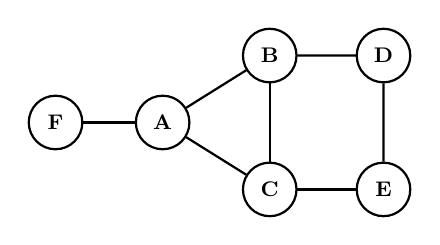
\begin{tikzpicture}[scale=0.85, every node/.style={transform shape}, cv/.style={draw, thick, circle, minimum size=8mm, inner sep=0pt, font=\small\bfseries}]
\node[cv] (A) at (0.00,1.20) {A};
\node[cv] (B) at (1.60,2.20) {B};
\node[cv] (C) at (1.60,0.20) {C};
\node[cv] (F) at (-1.60,1.20) {F};
\node[cv] (D) at (3.30,2.20) {D};
\node[cv] (E) at (3.30,0.20) {E};
\draw[thick] (A) to[] (B);
\draw[thick] (A) to[] (C);
\draw[thick] (A) to[] (F);
\draw[thick] (B) to[] (C);
\draw[thick] (B) to[] (D);
\draw[thick] (C) to[] (E);
\draw[thick] (D) to[] (E);
\end{tikzpicture}
\end{adjustbox}
\end{center}
\subq{(a)}A value is assigned to A and forward checking is run for A.
\begin{ansbox}[height=0.8cm]\end{ansbox}
\subq{(b)}A is assigned and forward checking is run; then B is assigned and forward checking is run for B.
\begin{ansbox}[height=0.8cm]\end{ansbox}
\subq{(c)}A is assigned and arc consistency is enforced.
\begin{ansbox}[height=0.8cm]\end{ansbox}
\subq{(d)}A is assigned and arc consistency is enforced; then B is assigned and arc consistency is enforced again.
\begin{ansbox}[height=1.2cm]\end{ansbox}
\clearpage
\question{11}Answer the following questions briefly.
\subq{(a)}Describe the ``laws of thought'' approach with a syllogism, and give the two obstacles the lecture mentions.
\begin{ansbox}[height=2.0cm]\end{ansbox}
\subq{(b)}On a 4-connected grid, compare the number of leaves of a depth-20 search tree with the number of distinct states within 20 steps (about $2d^2$). What does this say about tree-search vs graph-search?
\begin{ansbox}[height=1.8cm]\end{ansbox}
\subq{(c)}In simulated annealing a successor is $\Delta E=-3$ worse than the current state. Compute its acceptance probability at $T=10$, $3$, $1$. Why is simulated annealing better than plain hill climbing?
\begin{ansbox}[height=1.8cm]\end{ansbox}
\subq{(d)}With perfect move ordering, how many nodes does alpha-beta examine? Evaluate the effective branching factor for chess ($b\approx35$) and name two move-ordering techniques.
\begin{ansbox}[height=1.6cm]\end{ansbox}
\question{12}True or false?
For each statement, circle \textbf{T} or \textbf{F} and justify your answer in one or two sentences (an answer without a correct justification earns no credit).
\subq{1.}In graph search the frontier separates the expanded (interior) region from the unreached (exterior) region. \hfill \textbf{T \quad F}
\begin{ansbox}[height=1.5cm]\end{ansbox}
\subq{2.}For BFS, memory is a bigger problem than execution time. \hfill \textbf{T \quad F}
\begin{ansbox}[height=1.5cm]\end{ansbox}
\subq{3.}A* graph search with a consistent heuristic never needs to re-expand a state. \hfill \textbf{T \quad F}
\begin{ansbox}[height=1.5cm]\end{ansbox}
\subq{4.}A* with an inadmissible heuristic can never return an optimal solution. \hfill \textbf{T \quad F}
\begin{ansbox}[height=1.5cm]\end{ansbox}
\subq{5.}For the 8-puzzle, $h=\max\{2,h_{\text{Manhattan}}\}$ is admissible. \hfill \textbf{T \quad F}
\begin{ansbox}[height=1.5cm]\end{ansbox}
\subq{6.}For the 8-puzzle, $h=\min\{2,h_{\text{Manhattan}}\}$ is admissible. \hfill \textbf{T \quad F}
\begin{ansbox}[height=1.5cm]\end{ansbox}
\subq{7.}Pruning in expectimax is possible only if the leaf values are known to lie in a bounded range. \hfill \textbf{T \quad F}
\begin{ansbox}[height=1.5cm]\end{ansbox}
\subq{8.}In UCB1, increasing $C$ makes MCTS more exploratory. \hfill \textbf{T \quad F}
\begin{ansbox}[height=1.5cm]\end{ansbox}
\subq{9.}The least-constraining-value heuristic tries first the value that rules out the most choices for the neighbours. \hfill \textbf{T \quad F}
\begin{ansbox}[height=1.5cm]\end{ansbox}
\subq{10.}Any constraint over more than two variables can be transformed into binary constraints. \hfill \textbf{T \quad F}
\begin{ansbox}[height=1.5cm]\end{ansbox}
\end{document}